% !TEX root = catron-dissertation.tex
\epstopdfsetup{outdir=./images/04_dispersion_analysis/}

\chapter{Dispersion Analysis}
Dispersion analysis is an expansion of power spectra analysis from one-dimension to $n$-dimensions.
The technique allows a signal that is measured in both time and space to be separated into not only temporal-frequency components but also spacial-frequency components.
This allows not only the direction of travel that a particular wave to be determined but also the velocity of which that the wave travels.
The benefits of using a dispersion analysis are shown in Figure \ref{fig:04_dispersion_demo}.
\begin{figure}
\centering
  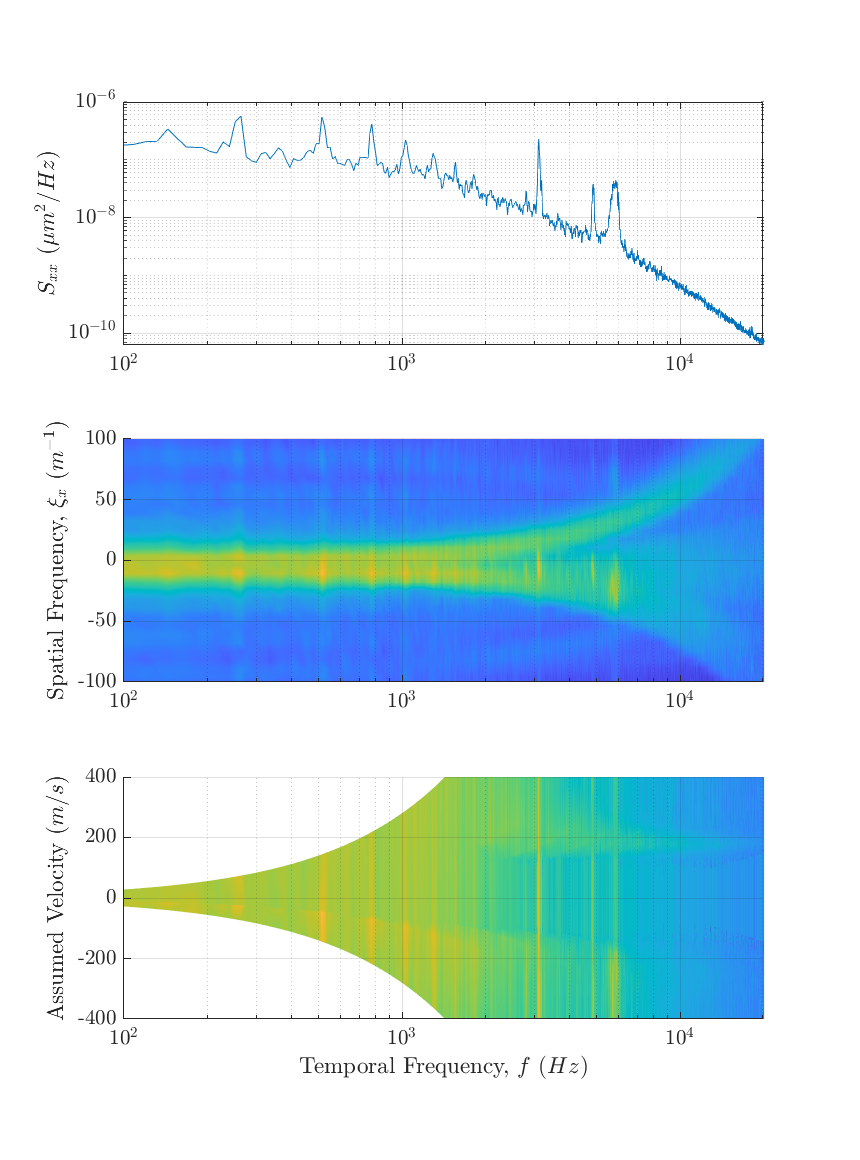
\includegraphics{../matlab/04_dispersion_analysis/dispersion_demo.eps}
  \caption{Dispersion plot example and comparison to traditional power spectra measurements. A single row of a wavefront measurement was used in this example. The top plot shows the typical power spectra measurement averaged over the entire row of data. Both the middle and bottom plots show the dispersion plot with the y-axis as spacial-frequency in the middle and velocity in the bottom assuming $u=f/\xi_x$.}
  \label{fig:04_dispersion_demo}
\end{figure}
The single row of sub-apertures from a wavefront measurement conducted with a 5-inch diameter beam propagating normally through two boundary layers with a free-stream Mach number of 0.5.
This measurement was preformed in the University of Notre Dame Whitefield Wind Tunnel in a test section that contained a model representing the fuselage of the AAOL aircraft \cite{Jumper-2013-8KtN3pue} with window that was flat and flush to the outer mold line of the fuselage.
The top plot shows a traditional power spectra representation averaged over the row of data.
Both the blade-passing frequency (517-Hz) and its sub-harmonic had similar power levels with an additional five harmonics showing significant spikes above the local baseline measurement.
There are three additional strong peaks at approximately 3100, 4850, and 5850 Hz that do not have an easily identifiable source or explanation.

Both the middle and bottom plots show a dispersion plot or two-dimensional power spectra measurement.
The colorbars were intentionally not shown in order to allow for all three plots to be aligned in the temporal frequency axis and the color space is representative of the power spectra in log-space.
The middle plot shows horizontally moving waves with the y-axis representing the spatial frequency, $\xi_x$, with units of inverse meters.
Waves with positive spatial frequencies are moving in the direction of flow.
All of the temporal frequency below 2000-Hz where the is an obvious separation between the upstream and downstream traveling optical disturbances are significantly more on the upstream traveling side.
The blade-passing frequency and its various harmonics show some significant broadband spatial frequency signals.
The three signals of unknown origin are clearly moving upstream but also show some significant broadband spatial signal that is indicative of a source producing optical disturbances that travel in both directions around the tunnel similar to the blade-passing frequency disturbances coming off of the wind tunnel fan.
In addition to optical disturbances branching off in the upstream and downstream moving directions there is a significant disturbances along zero spatial frequency representing a collection of standing waves.

The bottom plot shows the same dispersion plot as the middle one but with the y-axis representing an assumed velocity, $u_{assumed}$, where
\begin{equation}
  u_{assumed} = \frac{f}{\xi_x} \textrm{.}
  \label{eqn:04_velocity_assumed}
\end{equation}
The actual velocity, $u$, of a disturbance in the dispersion plot would be
\begin{equation}
  u = \frac{\partial f}{\partial \xi_x} \textrm{.}
  \label{eqn:04_velocity_actual}
\end{equation}
The assumed velocity measurement is in effect a average of the actual velocity assuming a zero-zero intercept in frequency space.
As there was no discernible separation between disturbance the upstream and downstream moving disturbances in the middle plot below 2000-Hz, there is no discernible velocity below that point.
The primary optical disturbance moving in the direction of flow is moving at the free-stream velocity of approximately 175-m/s.
The upstream traveling disturbance is traveling at the same speed but due to the signal being broader is more difficult to measure this way.
When the middle plot is shown with all linear axis, the slope of any given line through the origin is the inverse of the assumed velocity.
This is why the disturbances along the zero-spatial frequency line are a collection of standing waves and not some structure with broadband temporal content as it would be traveling at near infinite speed.
More discussion will follow a derivation of the dispersion analysis technique which is the n-dimensional power spectra.

\section{One-Dimensional Power Spectra Calculation}
The typical power spectra calculation on a set of data is only in one dimension.
This single dimension is often a time as would be the case when measuring a time series from a single sensor.
A sensor array used to take data at one moment in time could used to measure the power spectra in terms of spatial frequencies.
For a typical single-point measurement that varies in time, $x(t)$, the power spectra calculation is
\begin{equation}
 S_{xx} = \frac{|\fft(x(t))|^2}{N\cdot f_{s}} \textrm{,}
 \label{eqn:04_basic_sxx}
\end{equation}
where $\fft$ is the Fast Fourier Transform, $N$ is the number of samples, and $f_{s}$ is the sample rate.
For data that has only a real component the Fast Fourier Transform function produces magnitude and phase relations at each frequency step, $f_{s}/N$, over the range from zero-frequency up to but not including the Nyquist frequency, $f_s/w$, with a mirrored set of data that can be represented either below (starting at $-f_s/2$) or above (ending just below $f_s$) this range.
The Nyquist frequency not being included and the mirrored data is due to an assumption that is integral to the Fourier Transform, that being the signal is assumed to be periodic.

The total energy, $\sigma^2$, of the signal must be preserved through the transform from physical space-time to frequency space
\begin{equation}
  \sigma^2 = \frac{\sum x^2(t)}{N} = \Delta f\sum S_{xx}(f) \textrm{.}
  \label{eqn:04_fft_energy_conservation}
\end{equation}
Additionally, because of the periodic nature of the Fourier Transform and a finite sample length of discrete data, spectral leakage can cause the power in one frequency bin to leak into adjacent frequency bins.
To minimize this spectral leakage, windowing functions are employed which typically force the end points of the signal to zero.
The Hann window,
\begin{equation}
 w(t) = 1/2\left[1-\cos\left(\frac{2\pi t}{T}\right)\right] \textrm{,}
 \label{eqn:04_hann_window}
\end{equation}
is one of the more commonly used windowing functions where $w(t)$ is the window function, $t$ is the time at a given sample, and $T$ is the total sample time.
Since the windowing of a data set changes the signal energy some correction is needed to be applied.
For an arbitrary windowing function the correction factor, $c_w$, can be obtained by substituting the windowing function in place of $x(t)$ in Equation \ref{eqn:04_fft_energy_conservation},
\begin{equation}
 c_w = \frac{1}{\sqrt{\sum w^2(t)/N}} \textrm{.}
 \label{eqn:04_window_correction}
\end{equation}
For a Hann window this correction factor approaches $\sqrt{8/3}$ as $N$ goes to infinity.
When Equation \ref{eqn:04_basic_sxx} is combined with a windowing function and associated correction the double sided power spectra equation in one dimension becomes
\begin{equation}
 S_{xx} = \cdot\frac{|c_w\cdot\fft\{x(t)\cdot w(t)\}|^2}{N\cdot f_{s}} \textrm{.}
 \label{eqn:04_windowed_sxx}
\end{equation}
A simple MATLAB function for computing the power spectra of a one-dimension signal with an arbitrary windowing function is shown in Listing \ref{code:sc_simpleSXX}.

\section{N-Dimensional Power Spectra Calculation}
For measurements with multiple spatial and temporal dimensions the Fast Fourier Transform is just applied $n$-times where $n$ is the total number of dimensions, with each application in a different dimension,
\begin{equation}
 \fftn(x) = \fft(\fft(\cdots\fft(\fft(x,1),2)\cdots,n-1),n) \textrm{,}
 \label{eqn:04_fftn}
\end{equation}
where $\fft(x,n)$ is the Fast Fourier Transform of $x$ in the $n^{th}$ dimension.
For a $n$-dimensional array the power spectra the function becomes,
\begin{equation}
 \mathbf{S_{xx}} =c_w\cdot\frac{|\fftn\{f(\mathbf{x})\cdot w(\mathbf{x})\}|^2}{\prod{\overrightarrow{N}\cdot\overrightarrow{f_s}}} \textrm{,}
 \label{eqn:04_sxxn}
\end{equation}
where $\mathbf{S_{xx}}$ is the $n$-dimensional power spectra array or dispersion array, $f(\mathbf{x})$ is a $n$-dimensional set of data, $w(\mathbf{x})$ is a $n$-dimensional windowing function, $\overrightarrow{N}$ is a vector denoting the number of elements in each dimension, $\overrightarrow{f_s}$ is a vector denoting the sample rate in each dimension, and
\begin{equation}
 c_w = \frac{1}{\sqrt{\sum w^2(\mathbf{x})/\prod{\overrightarrow{N}}}} \textrm{.}
 \label{eqn:04_windown}
\end{equation}
The signal energy conservation relationship becomes
\begin{equation}
  \sigma^2=\frac{\sum\mathbf{x}}{\prod{\overrightarrow{N}}} = \prod{\overrightarrow{\Delta f_s}}\sum\mathbf{S_{xx}} \textrm{,}
  \label{eqn:04_fftn_energy_conservation}
\end{equation}
where $\overrightarrow{\Delta f_s}$ is a vector representing the frequency step sizes in each dimension.
A simple MATLAB code for calculating the dispersion of $x$ with an arbitrary windowing function is shown in Listing \ref{code:sc_simpleSXXn}.

\section{Non-Rectangular Spatial Windows}
For n-dimensional data sets that fill a rectangular array, a windowing function can easily be created by multiplying together a series of one-dimensional windowing functions created in the direction of each dimension.
For non-rectangular data sets, such as is often the case with optical wavefront measurement, windowing functions take some additional steps in there construction.
In cases when the spatial measurement locations are constant throughout time, the windowing function can be split into two separate components,
\begin{equation}
 w(\mathbf{x}) = w_t(t)\cdot w_s(x,y) \textrm{,}
 \label{eqn:04_window_sep}
\end{equation}
the temporal windowing function, $w_t(t)$, and the spatial windowing function, $w_s(x,y)$.
This paper uses a Hann window for the temporal windowing function and a modified Hann window for the spatial windowing function.
For the case of a circular aperture, the Hann window can be reformulated to be based normalized radius, $\rho_N$, of the aperture,
\begin{equation}
 w_s(\rho_N) =
 \begin{cases}
  \frac{1+\cos(\pi\cdot\rho_N)}{2} & \textrm{if } \rho_N < 1 \\
  0                                & \textrm{otherwise.}
 \end{cases}
 \label{eqn:04_window_space}
\end{equation}
This modified Hann window is two-dimensional with a value of one at the center of the aperture and decreases to zero at the edge of the aperture in the same manor as a Hann windows decreases from the center to either end.

Because the wavefronts used often had a clipped edge or other obscuration a different method was actually employed.
For an arbitrary shaped aperture, the minimum distance from any given measurement location to the edge of the aperture is used to create the spatial windows.
The minimum distance can be computed given the a set of points ($x$ and $y$) that spans the measurement range and the set of points outside of the aperture ($x_O$ and $y_O$),
\begin{equation}
 d_{min}(x,y) = \min\left\{\sqrt{(x-x_{O})^2+(y-y_{O})^2}\right\} \textrm{.}
 \label{eqn:04_window_space_arb_dist}
\end{equation}
This distance is then normalized by the maximum value and the resulting spatial window given a modified Hann window,
\begin{equation}
 w_s(x,y) = \frac{1+\cos\left\{\pi\cdot\left(1-d_{min}^{norm}(x,y)\right)\right\}}{2} \textrm{.}
 \label{eqn:04_window_space_arb}
\end{equation}
This same basic process can be extended to data sets where the locations of measurements in space vary with time.

\section{Dispersion Analysis}
At the beginning of this chapter a dispersion plot was shown along with a typical power spectra plot in Figure \ref{fig:04_dispersion_demo}.
This was for the purpose of doing a simple discussion of on some of the benefits of using a dispersion analysis on optical wavefronts.
That simple analysis was using only a single row of a wavefront and provided an incite into the disturbances that were moving in the horizontal direction only.
When a dispersion analysis is performed over all dimensions of a wavefront, as will be done for the remained of the chapter additional detail is available, additional detail as well as determination of optical disturbances moving vertically or any direction in between.
Figure \ref{fig:04_dispersion_comparison} shows a comparison between the two-dimensional single row dispersion and a three-dimensional dispersion showing the just the horizontal moving optical disturbances at both zero-vertical spatial frequency and the maximum value through all vertical spatial frequencies.
\begin{figure}
  \centering
  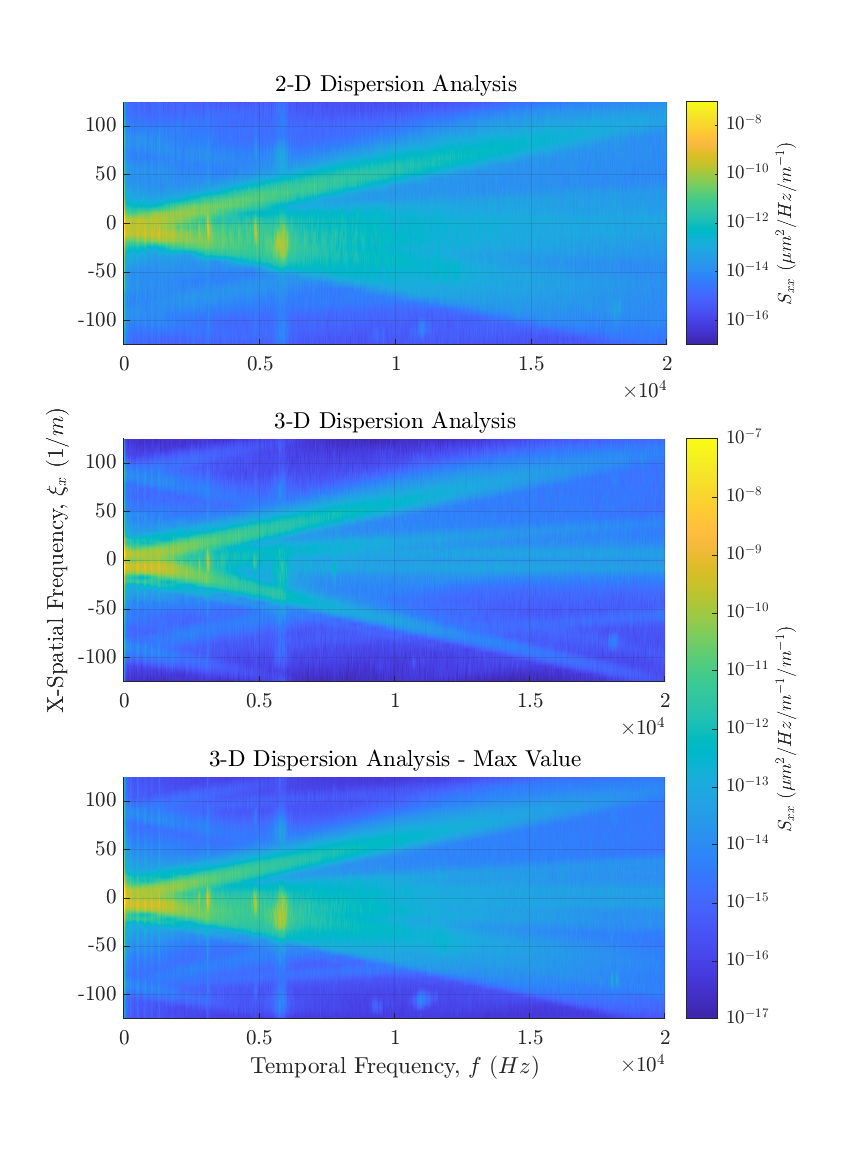
\includegraphics{../matlab/04_dispersion_analysis/dispersion_comparison.eps}
  \caption{Horizontal moving optical disturbances comparison. The top plot shows a two-dimensional dispersion analysis over a single row of data. The middle plot shows a three-dimensional dispersion analysis at $\xi_y=0$. The bottom plot shows the same three-dimensional dispersion analysis but showing the maximum value through the vertical axis.}
  \label{fig:04_dispersion_comparison}
\end{figure}
The top plots shows the two-dimensional dispersion plot that was previously shown in Figure \ref{fig:04_dispersion_demo} but this time with a linear temporal frequency axis.
The middle plot shows the three-dimensional dispersion plot at $\xi_y=0\ m^{-1}$, which shows a significant amount of additional data.
The two-dimensional dispersion shows a wide swath of signal that is generally traveling upstream from a line that goes through the origin and has a slight amount of positive slope downward to a line with a significant amount of negative slope.
This discussion of slopes is of the relative visible slope in the plots due and not actual slope calculation as the temporal frequency axis is several orders of magnitude larger than the spatial frequency axes (\textcolor{red}{footnote?}).

The slice of the full three-dimensional dispersion shows signal at the same limits for the two-dimensional swath of signal with some signal laying along the temporal frequency axis at $\xi_y=0\ m^{-1}$.
This signal represents a collection of stationary modes at each temporal frequency.
If this were to be some flow related phenomenon the velocity the disturbance would be nearing infinity.
On the three-dimensional dispersion plot there are easily observable signals that run parallel to the strongest signals but do not emanate from the origin.
These are signals that have been aliased due to the sample rate, either spatial or temporal, being to low.  This has some interesting implications in the possibility of being able to artificially increase the sample rate as will be discussed later.

The bottom plot of Figure \ref{fig:04_dispersion_comparison} shows the maximum value at each $f-\xi_x$ location through the range of $\xi_y$ values.
This effectively recreates the two-dimensional dispersion plot is a higher signal to noise ratio.
The aliased data is far more noticeable in this plot an in the two-dimensional one.
This indicates that a two-dimensional dispersion analysis is approximately the maximum value of the three-dimensional dispersion in a given dimension.
A reduced order dispersion can be calculated by
\begin{equation}
  S_{xx}^{n-1} = \max(S_{xx}^n,m)\cdot f_s^m \textrm{,}
\end{equation}
where $S_{xx}^n$ is the n-dimensional dispersion, $\max(x,m)$ is the maximum value of $x$ in the $m$-th dimension, and $f_s^m$ is the sample rate in the $m$-th dimension.
This can be shown in Figure \ref{fig:04_dispersion_max}.
The recovered power spectra from the two-dimensional dispersion analysis is a good estimation at the center of the frequency range but has some diversion near the edges.
It stays within half an order of magnitude below 1000-Hz with the signal peaks being a much closer approximation.
On the high end, the recovered power spectra has a decay rate that runs even with the direct computation up to about 10,000-Hz at which point the decay rate increases.
\begin{figure}
  \centering
  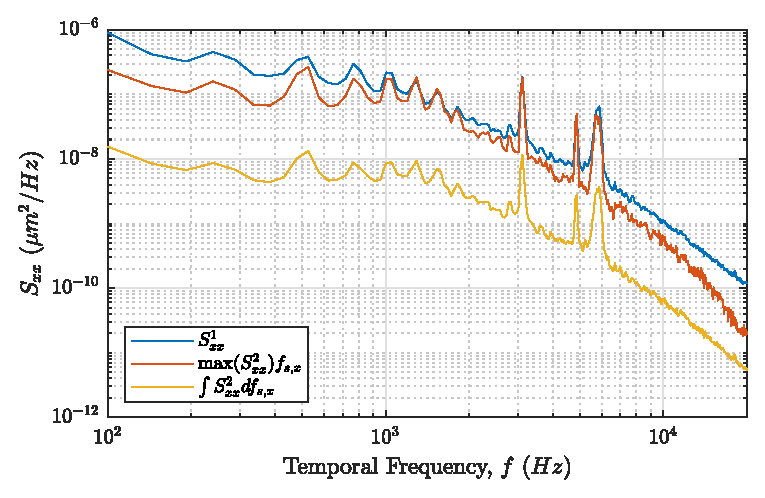
\includegraphics{../matlab/04_dispersion_analysis/dispersion_max.eps}
  \caption{Recovery of time-based power spectra from two-dimensional dispersion analysis.}
  \label{fig:04_dispersion_max}
\end{figure}

\subsection{2-D Slices of Full Dispersion}
The full dispersion analysis contains information of flow features not only moving in the horizontal direction as the two-dimensional dispersion showed but also in the vertical direction and the combinations of the two.
Figure \ref{fig:04_dispersion_xy} shows slices of the full dispersion in both the horizontal and vertical directions along with lines representing critical velocities.
Each of these plots is shown when the other spatial frequency is equal to zero, meaning that the disturbances shown are moving solely in that direction.
\begin{figure}
  \centering
  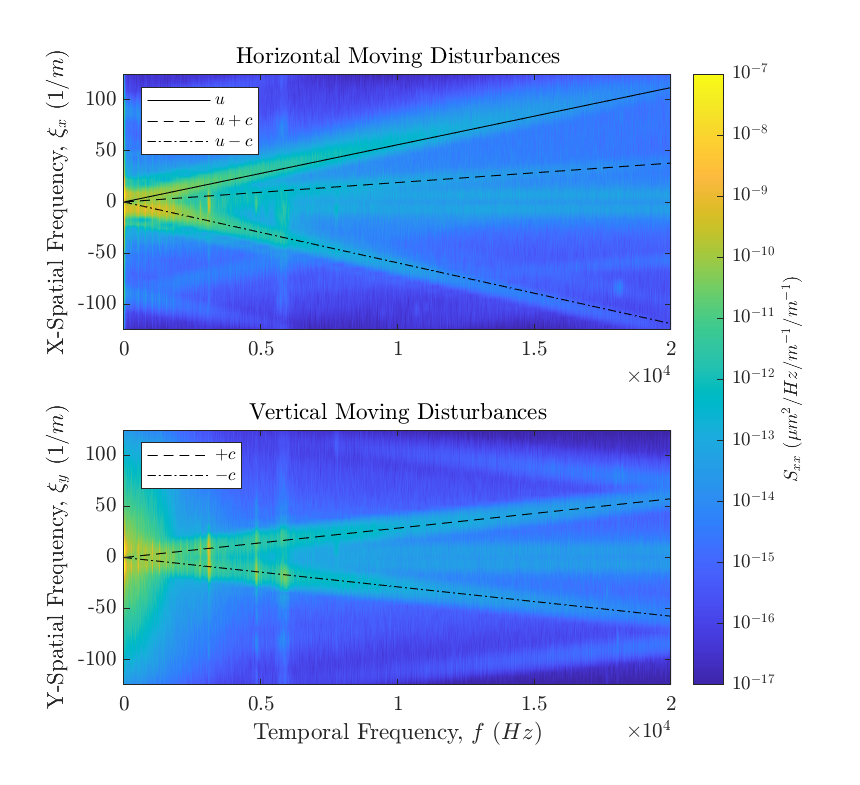
\includegraphics{../matlab/04_dispersion_analysis/dispersion_xy.eps}
  \caption{Horizontal and vertical moving optical disturbances. This is the same data as presented in Figure \ref{fig:04_dispersion_demo} but after calculating the full three-dimensional power spectra. The horizontal disturbances are shown at zero vertical spatial frequency and likewise the vertical disturbances are shown at zero horizontal spatial frequency.}
  \label{fig:04_dispersion_xy}
\end{figure}

The top plot shows the horizontally moving optical disturbances that has been shown previously.
There are three major flow related structures that can be observed.
The top most flow related structure is the boundary layers on both sides of the wind tunnel.
It can be seen that the boundary signal has a sharp drop off at the free-stream velocity, $u$, and has a slight decay as the velocity decreases (increasing slope).
Figure \ref{fig:04_dispersion_speed} shows the boundary layer velocity at a few cuts a little more clearly.
\begin{figure}
  \centering
  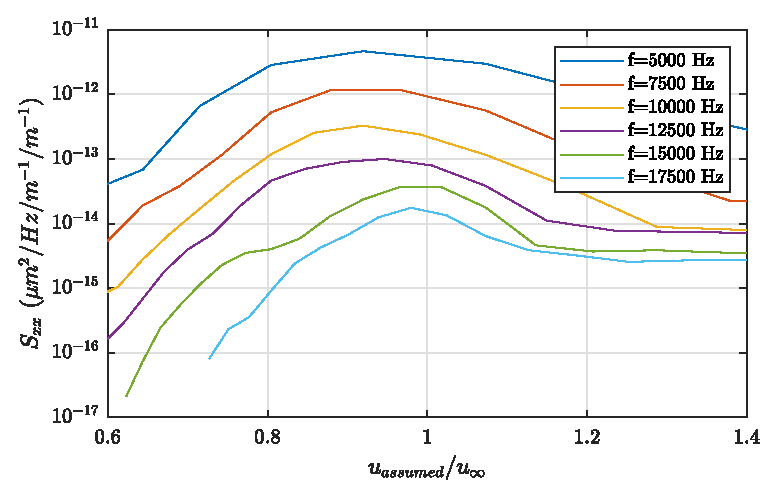
\includegraphics{../matlab/04_dispersion_analysis/dispersion_speed.eps}
  \caption{Assumed boundary speed at various temporal frequencies.}
  \label{fig:04_dispersion_speed}
\end{figure}
The boundary layer velocity has typically be reported as approximately 0.83$u$ \cite{Gordeyev-2014-jcJndkHM}.
This data shows the boundary layer velocity has a range of velocities at each given frequency in which the peak velocity component has some dependence on the temporal frequency.
The lower frequencies tend to have a lower velocity of around 0.9$u$ which is higher than has typically been reported while the higher frequencies approach the free-stream velocity.
When placing a lower bounding line on the boundary layer line in terms of speed in Figure \ref{fig:04_dispersion_xy}, a value of approximately 0.7$u$ seems to do a good job at bounding most of the boundary layer signal along with the free-stream velocity line.

The next two major flow related structures deal with acoustic signals traveling in both directions through the wind-tunnel.
The downstream traveling acoustic wave, $u+c$, typically has a low signal strength than the upstream traveling acoustic wave, $u-c$, due to the downstream traveling wave having a longer wavelength and thus more signal being filtered out due to aperture filtering \cite{Siegenthaler-2008-9Yutbt6c}.
At the low frequencies, the blade-passing frequency and its associated harmonics can be seen with regular spacing.
There also appears to be some constructive interference with the BPF and some of the aliased data around $\xi_x = \pm100\ m^{-1}$.

In both the horizontal and vertical moving plots the stationary modes are a prominent feature.
The two main features on the vertical moving disturbance plot is the signal at the speed of sound as well as some significant aliasing.
These to lines represent acoustic waves that are traversing either straight up or down.
Some of the high frequency spikes (~3, 5, and 6-kHz) seems to be laying along these speed of sound lines in the vertical direction and stationary in the horizontal direction.
These spikes maybe something in the test-section itself, along the top and bottom walls that is being excited and resonating.

\subsection{3-D Representations of Full Dispersion}
While the two-dimensional slices are fairly informative, particularly when it comes to signal strength of various flow structures and their velocities, a three-dimensional plot allows better visualization of the overall flow structures but some details are lost.
The same data that has been previously shown in slice form, is depicted in Figure \ref{fig:04_dispersion_3d} as an isosurface with a power of $10^{-14}$ $\mu m^2/Hz/m^{-1}/m^{-1}$ and shown from four different views.
\begin{figure}
  \centering
  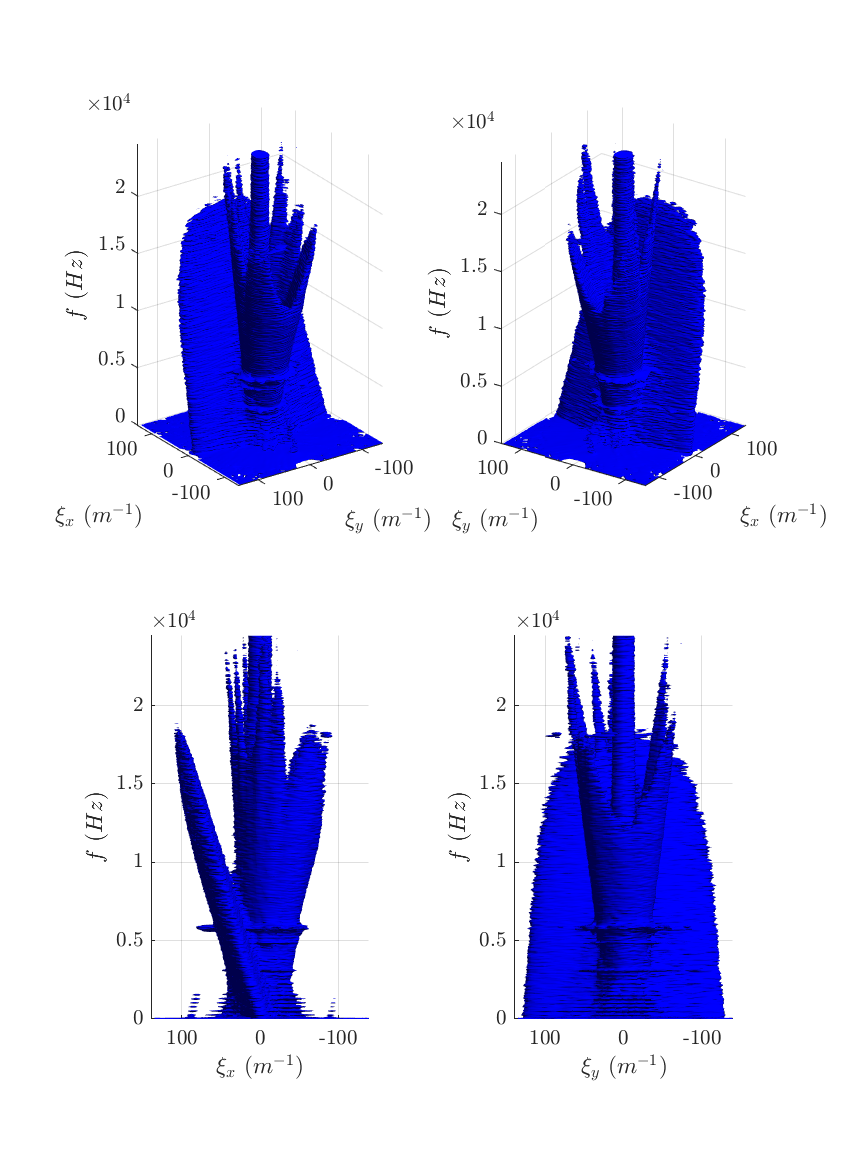
\includegraphics{../matlab/04_dispersion_analysis/dispersion_3d.eps}
  \caption{Three-dimensional view of the dispersion plot showing an isosurface at a power of $10^{-14}$ $\mu m^2/Hz/m^{-1}/m^{-1}$. The isosurface encompasses 99.9\% of the power of the wavefront.}
  \label{fig:04_dispersion_3d}
\end{figure}
This particular isosurface encompasses approximately 99.9\% of the power of the optical disturbances with little aliased information represented.
The largest feature is the boundary layer which resembles an ellipsoid or elliptical wing.
The other main feature is the acoustic signal which appears as a cone which has been tilted over a little bit.
The acoustic signal has several predominate spikes which form at high temporal frequencies indicating that there may be a small number of dominate duct modes.
The last feature is the stationary modes which have a near constant shape and magnitude through all frequency ranges.

Figure \ref{fig:04_dispersion_mach} shows two views of this three-dimensional dispersion but over a range of Mach numbers.
\begin{figure}
  \centering
  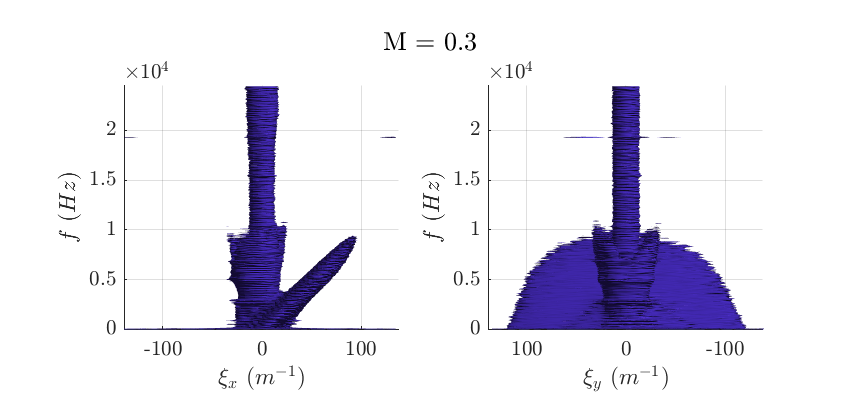
\includegraphics{../matlab/04_dispersion_analysis/dispersion_mach_0.3.eps}
  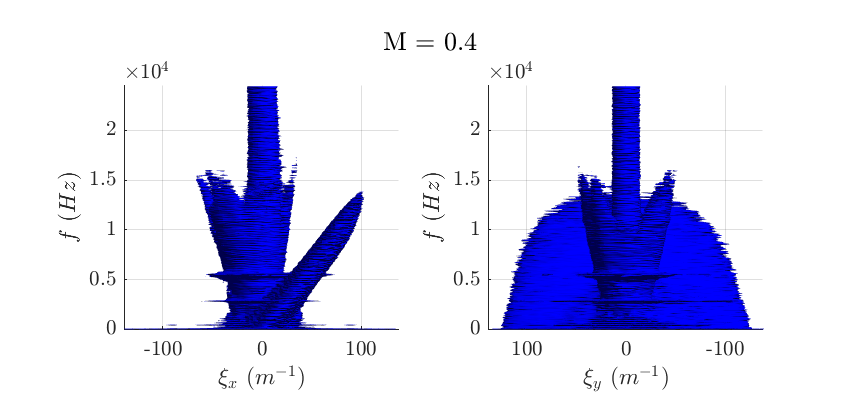
\includegraphics{../matlab/04_dispersion_analysis/dispersion_mach_0.4.eps}
  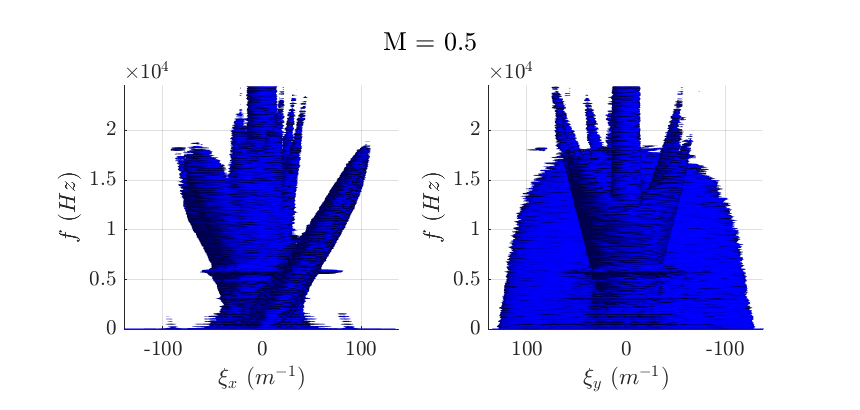
\includegraphics{../matlab/04_dispersion_analysis/dispersion_mach_0.5.eps}
  \caption{Three-dimensional view of dispersion plots as the Mach number increased from 0.3 to 0.5. The isosurfaces are all shown at a power of $10^{-14}$ $\mu m^2/Hz/m^{-1}/m^{-1}$ and all encompass 99.9\% of the wavefront power.}
  \label{fig:04_dispersion_mach}
\end{figure}
All of these plots are of an isosurface with the same strength as used in Figure \ref{fig:04_dispersion_3d}.
For a Mach number of 0.3, top plot, the most noticeable feature is the stationary modes which do not seem to change much as the Mach number is increase.
This indicates that the stationary waves are mostly as measurement artifact that could be from either laser or camera noise.
The boundary layer signal increases in power significantly as Mach number is increased but also the slope is significantly increased as well.
The acoustic signal sees some interesting evolution as well.
Along with the strength greatly increasing with Mach number, the slope of the upstream traveling disturbances decreases significantly while the downstream moving acoustic disturbances do not see much change other than an increase in signal strength.

While the three-dimensional views offer some significant incite, sometimes the insides need a close look a shown in Figure \ref{fig:04_dispersion_slices}.
\begin{figure}
  \centering
  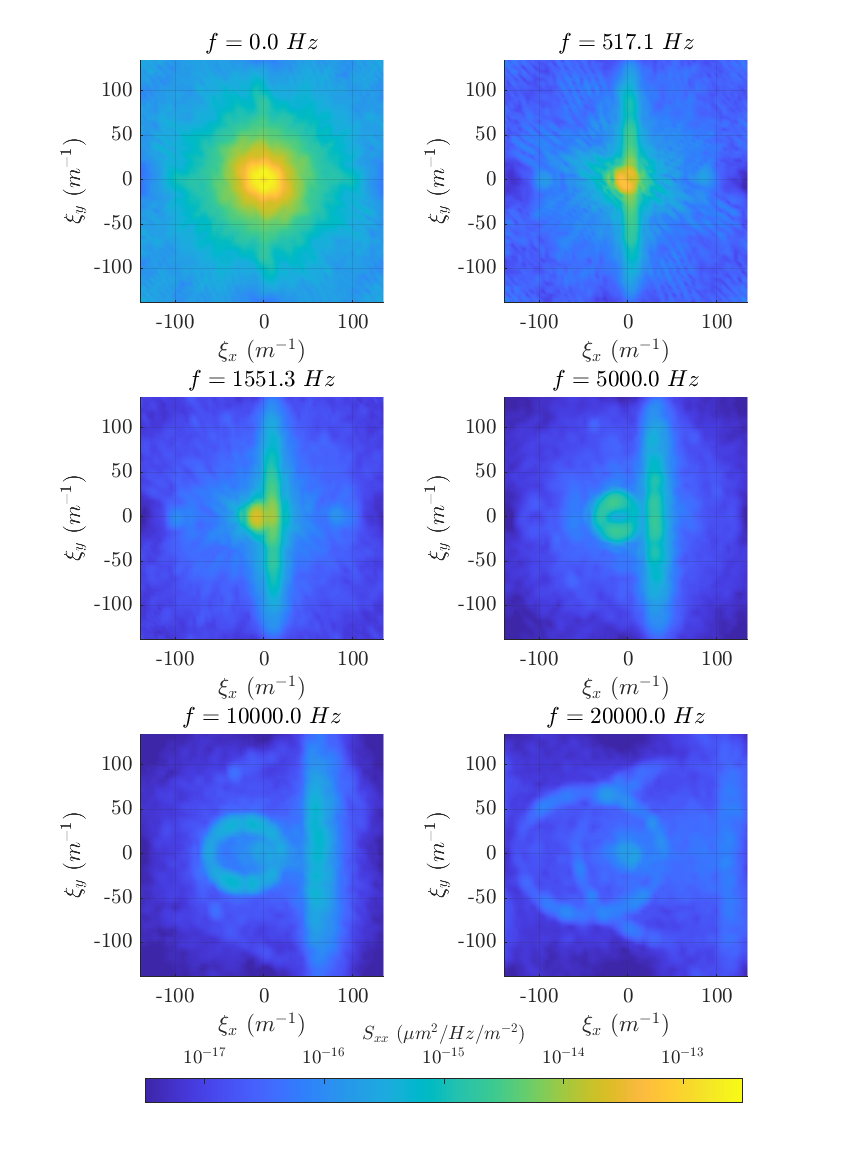
\includegraphics{../matlab/04_dispersion_analysis/dispersion_slices.eps}
  \caption{Additional dispersion slices at various temporal frequencies.}
  \label{fig:04_dispersion_slices}
\end{figure}
This figure shows slices of the dispersion array at several different temporal frequencies: a mean lensing slice at 0-Hz, the blade-passing frequency at 517-Hz, the second harmonic of the blade-passing frequency at 1551-Hz, and additional slices at 5, 10, and 20-kHz.
The mean lensing slice at 0-Hz shows a mostly axisymmetric pattern that is strongest in the center and dies out as the distance from the origin increases.
There appear to be the occasional spike radiating out from the center, most noticeably in line with the boundary layer signal.

The next four slices show boundary layers structure slowly moving towards positive x-spatial frequencies.
It does appear to be rotated slightly counter-clockwise indicating that the interrogation beam is slightly rotated between the test section and the wavefront sensor.
The boundary layers signal at the lower frequencies appears to be more elliptically shaped while the higher frequencies appear to have a sharp drop in signal strength going towards the origin and are slightly more feathered going away.
This could be indicative of lower frequency disturbances in the boundary layer typically traveling at a more uniform speed very near the free-stream velocity likely being either in the outer boundary layer or free-stream tunnel turbulence.
The higher frequency disturbances seem to have a wide range of velocities that approach the free-stream velocity and are likely small structures that span some significant portion of the boundary layer.

The acoustic disturbances show an interesting evolution as the frequency increase from fairly compact and strong signal just on the upstream traveling side of things around the blade-passing frequency to elliptical shaped rings at the higher frequencies.
At 20-kHz, there are two elliptical shapes that are easily identifiable, the smaller one is the signal that is actually present at that frequency while the other one is some aliased data due to a limited temporal sample rate.
The 10-kHz slice shows a little bit of acoustic aliasing
Both the 10 and 20-kHz acoustic rings show some favorable spatial frequencies which could also be seen in the three-dimensional view as spikes.
These two slices also show the center stationary modes that appear to be nearly identical.

\subsection{Artificially Increased Sample Rate}
Aliased data has been partially discussed previously.
When a signal crosses a plane represented by one of the Nyquist frequencies (positive or negative) it transposed to the conjugate Nyquist frequency plane and continues on with the same gradient as before, which is shown in Figure \ref{fig:04_dispersion_supersample} using the horizontal and vertical dispersion slices.
\begin{figure}
  \centering
  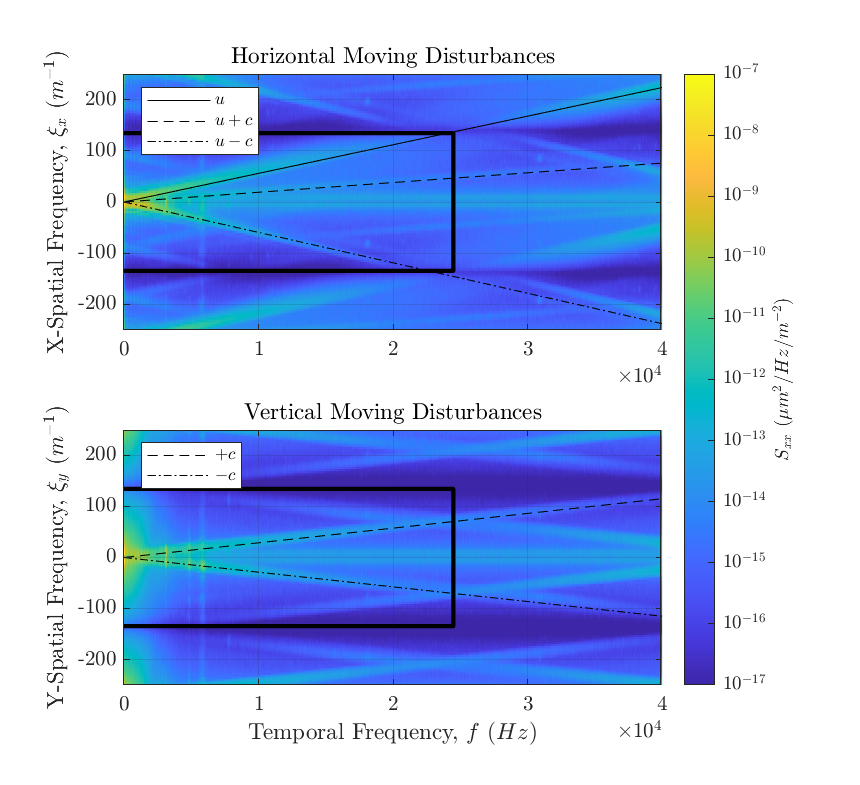
\includegraphics{../matlab/04_dispersion_analysis/dispersion_supersample.eps}
  \caption{Artificially increased temporal sample rate using a dispersion analysis. The black box represents original dispersion plot.}
  \label{fig:04_dispersion_supersample}
\end{figure}
Here the black box represents the original dispersion plot, while outside of that box is data that has an artificially increased sample rate.
This process can be accomplished by simply tiling the entire dispersion array in the desired dimension.
In this case the dispersion array was tiled in a three-by-three grid for each of the horizontal and vertical slices.
Along the spatial Nyquist frequency edges, there is a significant dip in the signal strength which would result in a spatial super sampling to have a significant loss of signal at these frequencies.

On the upstream moving disturbance side there is some noticeable aliasing that is present including a significant spike at 18-kHz (-80-$m^{-1}$) while aliased and about 31-kHz (-200-$m^{-1}$) when it has been unaliased.
As that upstream moving acoustic disturbance crosses the spatial Nyquist frequency, the signal strength drops significantly to local background levels.
The boundary layer signal is unfortunately to well aligned with its tiled self for any aliased data to be noticeable.
The vertically moving disturbances have some significant temporal aliasing but little to no spatial aliasing.

Just as the aliased signal is unaliased into the higher frequencies, non-aliased data is aliased into higher frequencies.
This means that some sort of filtering technique will need to be employed.
These filters should not only be designed to remove the aliased data from actual sample but also the aliased data from the super sampled frequencies.


% Depending of the sensor array construction, the signal could also be super sampled in the spatial dimensions as well.
% Because a Shack-Hartmann wavefront sensor is comprised of integrated measurements over each sub-aperture, artificially increasing the spatial sample rate is not possible due to the aperture filtering process.
%
% \begin{figure}
%   \centering
%   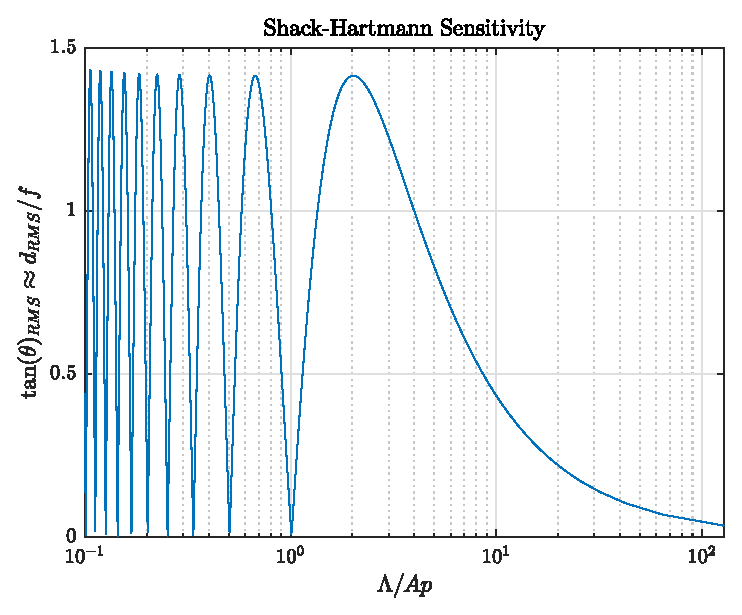
\includegraphics{../matlab/04_dispersion_analysis/shack_hartmann_sensitivity.eps}
%   \caption{Shack-Hartmann sensitivity as a function of the ratio of a structure's wavelength and the aperture size. This shows the RMS value of the displacement of the focal dot for a sub-aperture as a sinusoidal wave of unit magnitude passes through the sub-aperture.}
%   \label{fig:04_shack_hartmann_sensitivity}
% \end{figure}
